% In this talk, I’ll talk about how we can use silly games to understand the strengths and weaknesses of AIs. We first begin with games that test memory: testing the recall of obscure facts. While AI has been viewed as superhuman at this task, it isn’t universally so. We show that a new measure of adversarial datasets (the gap between humans and computers) is decreasing but not yet closed, with computers still struggling on abstract reasoning and knowing when they know the correct answer. Given these disparate skill sets, we then analyze how we can best build human and computer teams ito learn new facts and detect false statements. Finally, I close with a similar line of results for another silly language game, Diplomacy, where computers have still not reached dominance but can be used to assist human players think strategically and detect lies.”

\documentclass[compress]{beamer}

%\usepackage{beamerthemesplit}
\usepackage{xmpmulti}

\usepackage{booktabs}
\usepackage{xfrac}
\usepackage{graphicx,float,wrapfig, bbm}
\usepackage{amsfonts, bbold, comment}
\usepackage{mdwlist}
\usepackage{subfigure}
\usepackage{colortbl}
\usepackage{overpic}
\usepackage{pdfpages}
\usepackage[normalem]{ulem}
\usepackage{multirow}

\pgfdeclareimage[width=\paperwidth]{mybackground}{../../common/boulder.pdf}

\newcommand{\advscore}{\abr{AdvScore}}
\newcommand{\tif}[0]{\abr{tif}}
\newcommand{\twoplprob}[3]{ \frac{1}{1+\ex{-#3\left[ #1 - #2 \right] }  }}
\newcommand{\iif}{\abr{iif}}
\newcommand{\slda}[0]{\abr{slda}}
\newcommand{\bm}[1]{\mbox{\boldmath$#1$}}
\newcommand{\lda}[0]{\abr{lda}}
\newcommand{\explain}[2]{\underbrace{#2}_{\mbox{\footnotesize{#1}}}}
\newcommand{\itmspace}[0]{\hspace{2cm}}
\newcommand{\pos}[1]{{\texttt{#1}}}
\newcommand{\e}[2]{\mathbb{E}_{#1}\left[ #2 \right] }
\newcommand{\ind}[1]{\mathbb{I}\left[ #1 \right] }
\newcommand{\abr}[1]{\textsc{#1} }
\newcommand{\ex}[1]{\mbox{exp}\left\{ #1\right\} }
\newcommand{\g}{\, | \,}
\newcommand{\citename}[1]{#1 }
\newcommand{\fsi}[2]{
\begin{frame}[plain]
\vspace*{-1pt}
\makebox[\linewidth]{\includegraphics[width=\paperwidth]{#1}}
\begin{center}
#2
\end{center}
\end{frame}
}

\newcommand{\fsq}[3]{
\begin{frame}[plain]
\vspace*{-1pt}
\makebox[\linewidth]{\includegraphics[width=\paperwidth]{#1}}
\only<2->{
  \vspace{-4cm}
\begin{center}
  \begin{block}{#2}
    #3
    \end{block}
  \end{center}
  }
\end{frame}
}


\newcommand{\danquote}[1]{

\begin{flushright}
\begin{overpic}[width=5.5cm,tics=10]{general_figures/speech_bubble}
	\put(10,30) { \parbox{4cm}{#1 }}
\end{overpic}

\includegraphics[width=1.5cm]{general_figures/milkman_dan}
\end{flushright}
}


\newcommand{\gfxb}[2]{
	\begin{center}
		\includegraphics[width=#2\linewidth]{bs_in_ai/#1}
	\end{center}
}


\newcommand{\gfxm}[2]{
	\begin{center}
		\includegraphics[width=#2\linewidth]{muppet/#1}
	\end{center}
}


\newcommand{\gfxl}[2]{
\begin{center}
	\includegraphics[width=#2\linewidth]{mnemonic/#1}
\end{center}
}


\usetheme[
          showdate=true,                     % show the date on the title page
          alternativetitlepage=true,         % Use the fancy title page.
          titlepagelogo=general_figures/shell,              % Logo for the fir\
st page.
          ]{UMD}


\title[]{From Muppet Models to an an Interdisciplinary AI-first Education: Sustaining and Celebrating Maryland's AI Contributions}
\author{ Jordan Boyd-Graber}
\date{2025}

\institute[] % (optional, but mostly needed)
{University of Maryland}


%gets rid of bottom navigation symbols
\setbeamertemplate{navigation symbols}{}

%gets rid of footer
%will override 'frame number' instruction above
%comment out to revert to previous/default definitions
\setbeamertemplate{footline}{}

\begin{document}

\frame{
\titlepage
\tiny
}


\begin{frame}{AI at Maryland: Past, Present, and Future}

  \begin{columns}
    \column{.33\linewidth}
    \only<2->{\gfxm{mc_past}{1.0}}
    \only<5->{\begin{block}{\alert<8>{Past}}
        Maryland's Connection to Muppet Models
        \end{block}}
    \column{.33\linewidth}
    \only<3->{\gfxm{mc_present}{1.0}}
    \only<6->{\begin{block}{Present}
        Aligning AI with Educational Needs
        \end{block}}    
    \column{.33\linewidth}
    \only<4->{\gfxm{mc_future}{1.0}  }
        \only<7->{\begin{block}{Future}
            An AI Undergraduate Program
        \end{block}}
  \end{columns}

\end{frame}

\fsi{muppet/the_bad}{}

\fsi{muppet/family_tree}{}

\begin{frame}{Why Names Matter}

  \begin{block}{Gardner and Levy (1999)}
A name is more than the label employed to 
differentiate among the manufacturers of a
product. It is a complex symbol that represents a variety of ideas and attributes. It tells 
the consumers many things, not only by the 
way it sounds (and its literal meaning if it 
has one) but, more important, via the body
of associations it has built up and acquired.
\end{block}
\pause
\begin{block}{Grothendieck imagined\dots }
unknown and nameless worlds, crying out 
for me to become acquainted with them and 
bestow names upon them.
\end{block}

\end{frame}

\begin{frame}{Why not ``Large Language Models''?}

  \begin{columns}
    \column{.5\linewidth}
    \gfxm{clip}{1.0}
    \column{.5\linewidth}    
    \gfxm{chemistry}{1.0}
  \end{columns}
  \pause
  Models were pretty big before, and today models aren't just about language!
\end{frame}

\fsi{muppet/foundation_paper}{}

\fsq{muppet/crfm}{Foundations are Secure}{
  \begin{itemize}
  \item You should build on them
  \item They are secure
  \item You can trust them
  \end{itemize}
}

\fsq{muppet/newsom_frontier}{Bullock et al. (2024)}{there is no consistent definition of frontier models, and the term is sometimes deployed more for rhetorical effect than analytic clarity. }

\fsq{muppet/frontier_thesis}{McLure (2000)}{because the electronic frontier is still generally a lawless territory, vigilantism is often the preferred—and sometimes the only effective—response to what the cybersettlers perceive as crimes against both property and people}



\fsi{muppet/family_tree}{}
\fsi{muppet/snuffy_1}{}
\fsi{muppet/snuffy_2}{}


\fsi{muppet/muppet_show}{}

\begin{frame}{Why Muppet Models?}
\begin{itemize}
\item They’re fun
\item They’re interactive
  \item They are pretty accurate when tied to an underlying text
\item They’re multilingual
\item But they can still make stuff up
\item And they’re just a technically sophisticated solution
\item If you want a quality Muppet, you need to go through a large multinational corporation
\end{itemize}

\end{frame}

\fsi{muppet/next_time_cm}{}
\fsi{muppet/christmas}{}
\fsi{muppet/multilingual}{}
\fsi{muppet/allwissende_muellhalde}{}
\fsi{muppet/trashheap}{}
\fsi{muppet/creature_shop}{}
\fsi{muppet/underwater}{}
\fsi{muppet/erb_1}{}
\fsi{muppet/erb_2}{}
\fsi{muppet/moopets}{}

\begin{frame}{Why Muppet Models?}
\begin{itemize}
\item They’re fun
\item They’re interactive
  \item They are pretty accurate when tied to an underlying text
\item They’re multilingual
\item But they can still make stuff up
\item And they’re just a technically sophisticated solution
\item If you want a quality Muppet, you need to go through a large multinational corporation
  \pause
\item History and Maryland Pride
\end{itemize}
\end{frame}

\fsi{muppet/umd_1}{}
\fsi{muppet/umd_2}{}




\begin{frame}{AI at Maryland: Past, Present, and Future}

  \begin{columns}
    \column{.33\linewidth}
\gfxm{mc_past}{1.0}
\begin{block}{Past}
        Maryland's Connection to Muppet Models
        \end{block}
    \column{.33\linewidth}
\gfxm{mc_present}{1.0}
\begin{block}{\alert<2>{Present}}
        Aligning AI with Educational Needs
        \end{block}
    \column{.33\linewidth}
\gfxm{mc_future}{1.0}  
\begin{block}{Future}
            An AI Undergraduate Program
        \end{block}
  \end{columns}

\end{frame}


\begin{frame}{How Muppet Models are trained}
	
	\only<1>{\gfxl{llm_training}{1.0}}
	
	\only<1>{
		\begin{columns}
			\column{.3\linewidth}
			Learn to mimic human-written texts (next-token prediction)
			
			
			\column{.3\linewidth}
			Fine-tuned to be safe, follow instructions, use a certain style, \dots
			
			
			\column{.3\linewidth}
			Check the model’s knowledge, ability to help users, \dots
			
		\end{columns}
		
	}
	
	\only<2>{\gfxl{llm_training_zoom}{.8}}
	\only<3>{\gfxl{llm_zoom_1}{.8}}
	\only<4>{\gfxl{llm_zoom_2}{.8}}
	\only<5>{\gfxl{llm_zoom_3}{.8}}
	
\end{frame}

\fsi{mnemonic/sychophancy_paper}{}
\fsi{mnemonic/sychophancy_cartoon}{}


\begin{frame}{Helpfulness as Learning}
	\begin{columns}
		\column{.5\linewidth}
			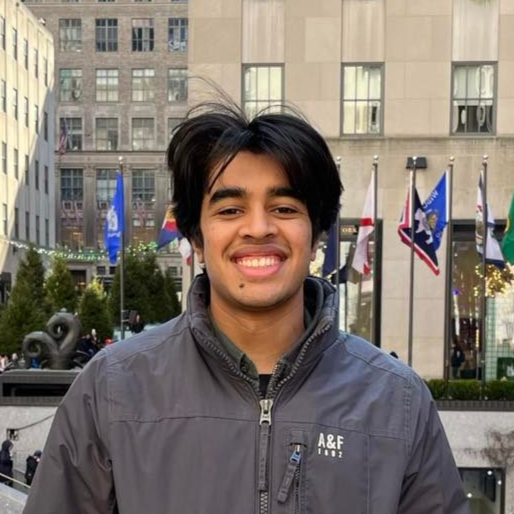
\includegraphics[width=.9\linewidth]{general_figures/nishant}
		\column{.5\linewidth}
			\gfxl{karl_paper}{.9}
			\gfxl{mnemonic_paper}{.9}
	\end{columns}
\end{frame}

\begin{frame}{Our Application: Learning Vocabulary}
	
	\gfxl{vocab}{.9}
\end{frame}

\begin{frame}{Using Mnmenonics to Learn}
	
	\gfxl{mnemonic}{.9}
	
	\textbf{Goal:} Build a mnemonic generator (SMART) to help students learn vocab
	
\end{frame}

\begin{frame}{Teach SMART which mnemonics are \textbf{helpful} via preference training}
	
	\gfxl{preference}{.9}
	
	Preference training assumes users can predict what is helpful \dots
	\pause
	but it's hard to know \textit{a priori} what works
	
\end{frame}

\begin{frame}{Flashcard Interface}
	
	47 Learners study with mnemonics from the SMART model in a flashcard app
	
	\only<1>{\gfxl{compliant_0}{.8}}
	\only<2>{\gfxl{compliant_1}{.8}}
	\only<3->{\gfxl{compliant_2}{.8}}
	\only<4>{\gfxl{compliant_correct}{.8}}
	
\end{frame}



\begin{frame}{Expressed Preferences: What users \textbf{think} will help them.}
	
	
	\only<1>{\gfxl{standard_preference_1}{.9}}
	\only<2>{\gfxl{standard_preference_2}{.9}}
	
\end{frame}


\begin{frame}{Do People Prefer What they Need?}
	
	\only<1>{\gfxl{preference_table_0}{.9}}
	\only<2>{\gfxl{preference_table_1}{.9}}
	\only<3>{\gfxl{preference_table_2}{.9}}
	\only<4>{\gfxl{preference_table_3}{.9}}
	
\end{frame}

\fsi{mnemonic/smart_system}{Learning, Model, Tuning}

\begin{frame}{Eval}
	
	\only<1>{\gfxl{eval_0}{.6}}
	\only<2>{\gfxl{eval_1}{.6}}
	\only<3->{\gfxl{eval_2}{.6}}
	
\end{frame}

\fsi{mnemonic/mnemonic_recap}{}


\begin{frame}{Bigger Picture}
  \begin{itemize}
  \item Rich synergies between education and AI research
  \item Measurement is a shared problem (item response theory)
  \item Other opportunities for measuring AI's helpfulness
    \begin{itemize}
    \item Coding
    \item Solving complicated questions
    \item Negotiation
    \item Detecting incorrect information
    \end{itemize}
    \pause
    \item The next generation of AI researchers needs to not just optimize loss functions but optimize for AI's role in society
  \end{itemize}
  
\end{frame}


\begin{frame}{AI at Maryland: Past, Present, and Future}

  \begin{columns}
    \column{.33\linewidth}
\gfxm{mc_past}{1.0}
\begin{block}{Past}
        Maryland's Connection to Muppet Models
        \end{block}
    \column{.33\linewidth}
\gfxm{mc_present}{1.0}
\begin{block}{Present}
        Aligning AI with Educational Needs
        \end{block}
    \column{.33\linewidth}
\gfxm{mc_future}{1.0}  
\begin{block}{\alert<2>{Future}}
            An AI Undergraduate Program
        \end{block}
  \end{columns}

\end{frame}



\begin{frame}{Why not just Computer Science?}

  \begin{columns}
    \column{.25\linewidth}
    \begin{block}{Too slow}
      Students get to AI in third or fourth year
    \end{block}
\pause
    \column{.25\linewidth}
    \begin{block}{Lack of shared prereqs}
      AI students need some common skills
    \end{block}
    \pause
    \column{.25\linewidth}
    \begin{block}{Differences}
      Focus on GPU, Python
    \end{block}
    \pause
    \column{.25\linewidth}
    \begin{block}{Connections}
      Options for interdisciplinary concentrations
    \end{block}
    
\end{columns}    
  \end{frame}



  \fsi{bs_in_ai/aim_logo}{}

  \fsi{bs_in_ai/pyret_banner}{}

  \fsi{bs_in_ai/pyret_test}{}

  \begin{frame}{Rethinking Systems Education}
    \gfxb{minitorch}{0.8}    
    \gfxb{gpu_memory}{0.8}
  \end{frame}

  \fsq{bs_in_ai/dependency}{Key Differences}{
    \begin{itemize}
    \item Pyret $\rightarrow$ Python
    \item AI Systems
    \item Required Ethics Course
    \item AI Fundamentals
    \item Statistics Focused on Ranking / Alignment
    \item Designing Fair Systems
    \end{itemize}
  }

  \begin{frame}{Connections Across Campus}
    \begin{itemize}
    \item AI, Society, and Decision Making: Information
    \item Generative AI: Arts and Humanities
    \item Robotics: Engineering
    \end{itemize}

    In addition to more traditional concentrations like AI Algorithms
    
  \end{frame}
 
\begin{frame}{AI at Maryland: Past, Present, and Future}

  \begin{columns}
    \column{.33\linewidth}
\gfxm{mc_past}{1.0}
\begin{block}{Past}
        Maryland's Connection to Muppet Models
        \end{block}
    \column{.33\linewidth}
\gfxm{mc_present}{1.0}
\begin{block}{Present}
        Aligning AI with Educational Needs
        \end{block}
    \column{.33\linewidth}
\gfxm{mc_future}{1.0}  
\begin{block}{Future}
            An AI Undergraduate Program
        \end{block}
  \end{columns}

\end{frame}




\end{document}
